% Options for packages loaded elsewhere
\PassOptionsToPackage{unicode}{hyperref}
\PassOptionsToPackage{hyphens}{url}
%
\documentclass[
]{book}
\usepackage{amsmath,amssymb}
\usepackage{lmodern}
\usepackage{iftex}
\ifPDFTeX
  \usepackage[T1]{fontenc}
  \usepackage[utf8]{inputenc}
  \usepackage{textcomp} % provide euro and other symbols
\else % if luatex or xetex
  \usepackage{unicode-math}
  \defaultfontfeatures{Scale=MatchLowercase}
  \defaultfontfeatures[\rmfamily]{Ligatures=TeX,Scale=1}
\fi
% Use upquote if available, for straight quotes in verbatim environments
\IfFileExists{upquote.sty}{\usepackage{upquote}}{}
\IfFileExists{microtype.sty}{% use microtype if available
  \usepackage[]{microtype}
  \UseMicrotypeSet[protrusion]{basicmath} % disable protrusion for tt fonts
}{}
\makeatletter
\@ifundefined{KOMAClassName}{% if non-KOMA class
  \IfFileExists{parskip.sty}{%
    \usepackage{parskip}
  }{% else
    \setlength{\parindent}{0pt}
    \setlength{\parskip}{6pt plus 2pt minus 1pt}}
}{% if KOMA class
  \KOMAoptions{parskip=half}}
\makeatother
\usepackage{xcolor}
\IfFileExists{xurl.sty}{\usepackage{xurl}}{} % add URL line breaks if available
\IfFileExists{bookmark.sty}{\usepackage{bookmark}}{\usepackage{hyperref}}
\hypersetup{
  pdftitle={Libro sobre VirusTotal},
  pdfauthor={Antonio Molina Baena y Francisco José García Barbero},
  hidelinks,
  pdfcreator={LaTeX via pandoc}}
\urlstyle{same} % disable monospaced font for URLs
\usepackage{color}
\usepackage{fancyvrb}
\newcommand{\VerbBar}{|}
\newcommand{\VERB}{\Verb[commandchars=\\\{\}]}
\DefineVerbatimEnvironment{Highlighting}{Verbatim}{commandchars=\\\{\}}
% Add ',fontsize=\small' for more characters per line
\usepackage{framed}
\definecolor{shadecolor}{RGB}{248,248,248}
\newenvironment{Shaded}{\begin{snugshade}}{\end{snugshade}}
\newcommand{\AlertTok}[1]{\textcolor[rgb]{0.94,0.16,0.16}{#1}}
\newcommand{\AnnotationTok}[1]{\textcolor[rgb]{0.56,0.35,0.01}{\textbf{\textit{#1}}}}
\newcommand{\AttributeTok}[1]{\textcolor[rgb]{0.77,0.63,0.00}{#1}}
\newcommand{\BaseNTok}[1]{\textcolor[rgb]{0.00,0.00,0.81}{#1}}
\newcommand{\BuiltInTok}[1]{#1}
\newcommand{\CharTok}[1]{\textcolor[rgb]{0.31,0.60,0.02}{#1}}
\newcommand{\CommentTok}[1]{\textcolor[rgb]{0.56,0.35,0.01}{\textit{#1}}}
\newcommand{\CommentVarTok}[1]{\textcolor[rgb]{0.56,0.35,0.01}{\textbf{\textit{#1}}}}
\newcommand{\ConstantTok}[1]{\textcolor[rgb]{0.00,0.00,0.00}{#1}}
\newcommand{\ControlFlowTok}[1]{\textcolor[rgb]{0.13,0.29,0.53}{\textbf{#1}}}
\newcommand{\DataTypeTok}[1]{\textcolor[rgb]{0.13,0.29,0.53}{#1}}
\newcommand{\DecValTok}[1]{\textcolor[rgb]{0.00,0.00,0.81}{#1}}
\newcommand{\DocumentationTok}[1]{\textcolor[rgb]{0.56,0.35,0.01}{\textbf{\textit{#1}}}}
\newcommand{\ErrorTok}[1]{\textcolor[rgb]{0.64,0.00,0.00}{\textbf{#1}}}
\newcommand{\ExtensionTok}[1]{#1}
\newcommand{\FloatTok}[1]{\textcolor[rgb]{0.00,0.00,0.81}{#1}}
\newcommand{\FunctionTok}[1]{\textcolor[rgb]{0.00,0.00,0.00}{#1}}
\newcommand{\ImportTok}[1]{#1}
\newcommand{\InformationTok}[1]{\textcolor[rgb]{0.56,0.35,0.01}{\textbf{\textit{#1}}}}
\newcommand{\KeywordTok}[1]{\textcolor[rgb]{0.13,0.29,0.53}{\textbf{#1}}}
\newcommand{\NormalTok}[1]{#1}
\newcommand{\OperatorTok}[1]{\textcolor[rgb]{0.81,0.36,0.00}{\textbf{#1}}}
\newcommand{\OtherTok}[1]{\textcolor[rgb]{0.56,0.35,0.01}{#1}}
\newcommand{\PreprocessorTok}[1]{\textcolor[rgb]{0.56,0.35,0.01}{\textit{#1}}}
\newcommand{\RegionMarkerTok}[1]{#1}
\newcommand{\SpecialCharTok}[1]{\textcolor[rgb]{0.00,0.00,0.00}{#1}}
\newcommand{\SpecialStringTok}[1]{\textcolor[rgb]{0.31,0.60,0.02}{#1}}
\newcommand{\StringTok}[1]{\textcolor[rgb]{0.31,0.60,0.02}{#1}}
\newcommand{\VariableTok}[1]{\textcolor[rgb]{0.00,0.00,0.00}{#1}}
\newcommand{\VerbatimStringTok}[1]{\textcolor[rgb]{0.31,0.60,0.02}{#1}}
\newcommand{\WarningTok}[1]{\textcolor[rgb]{0.56,0.35,0.01}{\textbf{\textit{#1}}}}
\usepackage{longtable,booktabs,array}
\usepackage{calc} % for calculating minipage widths
% Correct order of tables after \paragraph or \subparagraph
\usepackage{etoolbox}
\makeatletter
\patchcmd\longtable{\par}{\if@noskipsec\mbox{}\fi\par}{}{}
\makeatother
% Allow footnotes in longtable head/foot
\IfFileExists{footnotehyper.sty}{\usepackage{footnotehyper}}{\usepackage{footnote}}
\makesavenoteenv{longtable}
\usepackage{graphicx}
\makeatletter
\def\maxwidth{\ifdim\Gin@nat@width>\linewidth\linewidth\else\Gin@nat@width\fi}
\def\maxheight{\ifdim\Gin@nat@height>\textheight\textheight\else\Gin@nat@height\fi}
\makeatother
% Scale images if necessary, so that they will not overflow the page
% margins by default, and it is still possible to overwrite the defaults
% using explicit options in \includegraphics[width, height, ...]{}
\setkeys{Gin}{width=\maxwidth,height=\maxheight,keepaspectratio}
% Set default figure placement to htbp
\makeatletter
\def\fps@figure{htbp}
\makeatother
\setlength{\emergencystretch}{3em} % prevent overfull lines
\providecommand{\tightlist}{%
  \setlength{\itemsep}{0pt}\setlength{\parskip}{0pt}}
\setcounter{secnumdepth}{5}
\usepackage{booktabs}
\usepackage{booktabs}
\usepackage{longtable}
\usepackage{array}
\usepackage{multirow}
\usepackage{wrapfig}
\usepackage{float}
\usepackage{colortbl}
\usepackage{pdflscape}
\usepackage{tabu}
\usepackage{threeparttable}
\usepackage{threeparttablex}
\usepackage[normalem]{ulem}
\usepackage{makecell}
\usepackage{xcolor}
\ifLuaTeX
  \usepackage{selnolig}  % disable illegal ligatures
\fi
\usepackage[]{natbib}
\bibliographystyle{plainnat}

\title{Libro sobre VirusTotal}
\author{Antonio Molina Baena y Francisco José García Barbero}
\date{2022-05-27}

\begin{document}
\maketitle

{
\setcounter{tocdepth}{1}
\tableofcontents
}
\hypertarget{json}{%
\chapter{Json}\label{json}}

En este apartado veremos la creacion de un dataframe leyendo los json

\hypertarget{covertir-json-a-dataframe}{%
\section{Covertir json a dataframe}\label{covertir-json-a-dataframe}}

Cargamos las librerias que vamos a usar durante el proyecto:

library(jsonlite)
library(curl)
library(tidyjson)
library(dplyr)
library(purrr)
library(tidyverse)
library(jsonlite)
library(rjson)
library(fcaR)
library(parallel)
library(rlist)
library(kableExtra)
library(factoextra)
library(fpc)
library(hasseDiagram)
library(plotly)
library(dash)
library(dashCoreComponents)
library(dashHtmlComponents)
library(ggfortify)
library(ggdendro)
library(heatmaply)

Ruta de trabajo

\begin{Shaded}
\begin{Highlighting}[]
\FunctionTok{setwd}\NormalTok{(}\StringTok{"\textasciitilde{}/Laboratorio/Book trabajo vt/Android/Android"}\NormalTok{)}
\CommentTok{\#path \textless{}{-} "\textasciitilde{}/Laboratorio/Book trabajo vt/Android/Android"}
\NormalTok{path }\OtherTok{\textless{}{-}} \StringTok{"./"}
\CommentTok{\# Creamos una lista con todos los json que hay en el directorio}

\NormalTok{files }\OtherTok{\textless{}{-}} \FunctionTok{list.files}\NormalTok{()}

\FunctionTok{library}\NormalTok{(parallel)}
\NormalTok{cl }\OtherTok{\textless{}{-}} \FunctionTok{makeCluster}\NormalTok{(}\FunctionTok{detectCores}\NormalTok{() }\SpecialCharTok{{-}} \DecValTok{1}\NormalTok{)}
\NormalTok{json\_list}\OtherTok{\textless{}{-}}\FunctionTok{parLapply}\NormalTok{(cl,files,}\ControlFlowTok{function}\NormalTok{(x) jsonlite}\SpecialCharTok{::}\FunctionTok{read\_json}\NormalTok{(}\AttributeTok{path =}\NormalTok{ x, }\AttributeTok{simplifyVector =} \ConstantTok{TRUE}\NormalTok{))}
\FunctionTok{stopCluster}\NormalTok{(cl)}

\FunctionTok{class}\NormalTok{(json\_list)}
\end{Highlighting}
\end{Shaded}

\begin{verbatim}
## [1] "list"
\end{verbatim}

\begin{Shaded}
\begin{Highlighting}[]
\NormalTok{t1 }\OtherTok{\textless{}{-}}\NormalTok{ json\_list }\SpecialCharTok{\%\textgreater{}\%}\NormalTok{ gather\_object}
\NormalTok{t1}
\end{Highlighting}
\end{Shaded}

\begin{verbatim}
## # A tbl_json: 5,124 x 3 tibble with a "JSON" attribute
##    ..JSON                  document.id name            
##    <chr>                         <int> <chr>           
##  1 "\"f6e2a738ceacee..."             1 vhash           
##  2 "\"/vdepot/apk/42..."             1 submission_names
##  3 "\"2021-11-03 08:..."             1 scan_date       
##  4 "\"2021-11-03 08:..."             1 first_seen      
##  5 "61"                              1 total           
##  6 "{\"exiftool\":{\"M..."           1 additional_info 
##  7 "1956125"                         1 size            
##  8 "null"                            1 authentihash    
##  9 "1"                               1 times_submitted 
## 10 "0"                               1 harmless_votes  
## # ... with 5,114 more rows
\end{verbatim}

\begin{Shaded}
\begin{Highlighting}[]
\NormalTok{json\_tabla }\OtherTok{\textless{}{-}}\NormalTok{ json\_list }\SpecialCharTok{\%\textgreater{}\%}
  \FunctionTok{spread\_all}\NormalTok{()}
\NormalTok{json\_tabla}
\end{Highlighting}
\end{Shaded}

\begin{verbatim}
## # A tbl_json: 183 x 1,122 tibble with a "JSON" attribute
##    ..JSON   document.id vhash submission_names scan_date first_seen total   size
##    <chr>          <int> <chr> <chr>            <chr>     <chr>      <dbl>  <dbl>
##  1 "{\"vha~           1 f6e2~ /vdepot/apk/42/~ 2021-11-~ 2021-11-0~    61 1.96e6
##  2 "{\"vha~           2 c33f~ 398e6e8146d6147~ 2021-11-~ 2021-11-0~    61 2.67e6
##  3 "{\"vha~           3 1a58~ 07d00b70d7f6.zip 2021-11-~ 2021-11-0~    61 4.00e6
##  4 "{\"vha~           4 adf3~ <NA>             2021-11-~ 2015-01-2~    64 5.00e5
##  5 "{\"vha~           5 f6e2~ /vdepot/apk/CD/~ 2021-11-~ 2021-11-0~    62 1.96e6
##  6 "{\"vha~           6 e289~ ff6f1dd413e4.zip 2021-11-~ 2021-11-0~    61 4.14e6
##  7 "{\"vha~           7 <NA>  b8456ae6435a76b~ 2021-11-~ 2021-06-0~    61 3.03e6
##  8 "{\"vha~           8 c33f~ 511a4359f936ffc~ 2021-11-~ 2021-11-0~    60 2.67e6
##  9 "{\"vha~           9 c33f~ ed89d9884a455e4~ 2021-11-~ 2021-11-0~    60 2.67e6
## 10 "{\"vha~          10 <NA>  <NA>             2021-11-~ 2017-11-2~    60 5.88e3
## # ... with 173 more rows, and 1,114 more variables: authentihash <lgl>,
## #   times_submitted <dbl>, harmless_votes <dbl>, malicious_votes <dbl>,
## #   sha256 <chr>, type <chr>, tags <chr>, scan_id <chr>, unique_sources <dbl>,
## #   positives <dbl>, ssdeep <chr>, md5 <chr>, permalink <chr>, sha1 <chr>,
## #   response_code <dbl>, community_reputation <dbl>, verbose_msg <chr>,
## #   last_seen <chr>, ITW_urls <chr>, additional_info.trid <chr>,
## #   additional_info.magic <chr>, submission.submitter_region <chr>, ...
\end{verbatim}

\begin{Shaded}
\begin{Highlighting}[]
\NormalTok{json\_tabla\_no\_na }\OtherTok{\textless{}{-}}\NormalTok{ json\_tabla }\SpecialCharTok{\%\textgreater{}\%} \FunctionTok{select\_if}\NormalTok{(}\SpecialCharTok{\textasciitilde{}!}\FunctionTok{all}\NormalTok{(}\FunctionTok{is.na}\NormalTok{(.)))}
\end{Highlighting}
\end{Shaded}

\hypertarget{reglas-de-asociaciuxf3n}{%
\chapter{Reglas de asociación}\label{reglas-de-asociaciuxf3n}}

Usando la tabla sin na selecciono alguna

Usando apriori con supp 0.01

\begin{Shaded}
\begin{Highlighting}[]
\NormalTok{r1 }\OtherTok{\textless{}{-}} \FunctionTok{apriori}\NormalTok{(tabla\_RA,  }\AttributeTok{parameter =} \FunctionTok{list}\NormalTok{(}\AttributeTok{supp =} \FloatTok{0.01}\NormalTok{, }\AttributeTok{conf =} \FloatTok{0.5}\NormalTok{,}\AttributeTok{minlen=}\DecValTok{2}\NormalTok{))}
\end{Highlighting}
\end{Shaded}

\begin{verbatim}
## Warning: Column(s) 1, 2, 3, 4, 5, 6 not logical or factor. Applying default
## discretization (see '? discretizeDF').
\end{verbatim}

\begin{verbatim}
## Apriori
## 
## Parameter specification:
##  confidence minval smax arem  aval originalSupport maxtime support minlen
##         0.5    0.1    1 none FALSE            TRUE       5    0.01      2
##  maxlen target  ext
##      10  rules TRUE
## 
## Algorithmic control:
##  filter tree heap memopt load sort verbose
##     0.1 TRUE TRUE  FALSE TRUE    2    TRUE
## 
## Absolute minimum support count: 0 
## 
## set item appearances ...[0 item(s)] done [0.00s].
## set transactions ...[138 item(s), 71 transaction(s)] done [0.00s].
## sorting and recoding items ... [138 item(s)] done [0.00s].
## creating transaction tree ... done [0.00s].
## checking subsets of size 1 2 3 4 5 6 done [0.00s].
## writing ... [6583 rule(s)] done [0.00s].
## creating S4 object  ... done [0.00s].
\end{verbatim}

\begin{Shaded}
\begin{Highlighting}[]
\FunctionTok{inspect}\NormalTok{(}\FunctionTok{head}\NormalTok{(r1))}
\end{Highlighting}
\end{Shaded}

\begin{verbatim}
##     lhs                                                   rhs                                                               support confidence   coverage      lift count
## [1] {scans.McAfee.result=Artemis!C5B53B908443}         => {scans.CAT-QuickHeal.result=Android.SMSReg.A (PUP)}            0.01408451          1 0.01408451  6.454545     1
## [2] {scans.McAfee.result=Artemis!C5B53B908443}         => {scans.Lionic.result=Riskware.AndroidOS.SMSreg.z!c}            0.01408451          1 0.01408451  6.454545     1
## [3] {scans.McAfee.result=Artemis!C5B53B908443}         => {scans.ESET-NOD32.result=Android/SMSreg.UA potentially unsafe} 0.01408451          1 0.01408451  6.454545     1
## [4] {scans.McAfee.result=Artemis!C5B53B908443}         => {submission.submitter_country=CA}                              0.01408451          1 0.01408451  1.918919     1
## [5] {scans.McAfee.result=Artemis!C5B53B908443}         => {additional_info.exiftool.FileType=ZIP}                        0.01408451          1 0.01408451  1.000000     1
## [6] {scans.CAT-QuickHeal.result=Android.Agent.GEN1478} => {scans.McAfee.result=Artemis!433E1FBFF2F2}                     0.01408451          1 0.01408451 71.000000     1
\end{verbatim}

\begin{Shaded}
\begin{Highlighting}[]
\NormalTok{r2 }\OtherTok{\textless{}{-}} \FunctionTok{sort}\NormalTok{(r1,}\AttributeTok{by=}\StringTok{"support"}\NormalTok{)}
\FunctionTok{inspect}\NormalTok{(}\FunctionTok{head}\NormalTok{(r2,}\DecValTok{5}\NormalTok{))}
\end{Highlighting}
\end{Shaded}

\begin{verbatim}
##     lhs                                                 rhs                                                support confidence  coverage     lift count
## [1] {submission.submitter_country=CA}                => {additional_info.exiftool.FileType=ZIP}          0.5211268  1.0000000 0.5211268 1.000000    37
## [2] {additional_info.exiftool.FileType=ZIP}          => {submission.submitter_country=CA}                0.5211268  0.5211268 1.0000000 1.000000    37
## [3] {scans.Lionic.result=Adware.AndroidOS.Ewind.A!c} => {submission.submitter_country=CA}                0.3380282  1.0000000 0.3380282 1.918919    24
## [4] {submission.submitter_country=CA}                => {scans.Lionic.result=Adware.AndroidOS.Ewind.A!c} 0.3380282  0.6486486 0.5211268 1.918919    24
## [5] {scans.Lionic.result=Adware.AndroidOS.Ewind.A!c} => {additional_info.exiftool.FileType=ZIP}          0.3380282  1.0000000 0.3380282 1.000000    24
\end{verbatim}

\hypertarget{usando-arulesviz}{%
\section{Usando arulesViz}\label{usando-arulesviz}}

Visualizamos graficamente las reglas

\begin{Shaded}
\begin{Highlighting}[]
\FunctionTok{library}\NormalTok{(arulesViz)}
\NormalTok{cabesa}\OtherTok{\textless{}{-}} \FunctionTok{head}\NormalTok{(r1,}\DecValTok{100}\NormalTok{)}
\FunctionTok{plot}\NormalTok{(cabesa)}
\end{Highlighting}
\end{Shaded}

\begin{verbatim}
## To reduce overplotting, jitter is added! Use jitter = 0 to prevent jitter.
\end{verbatim}

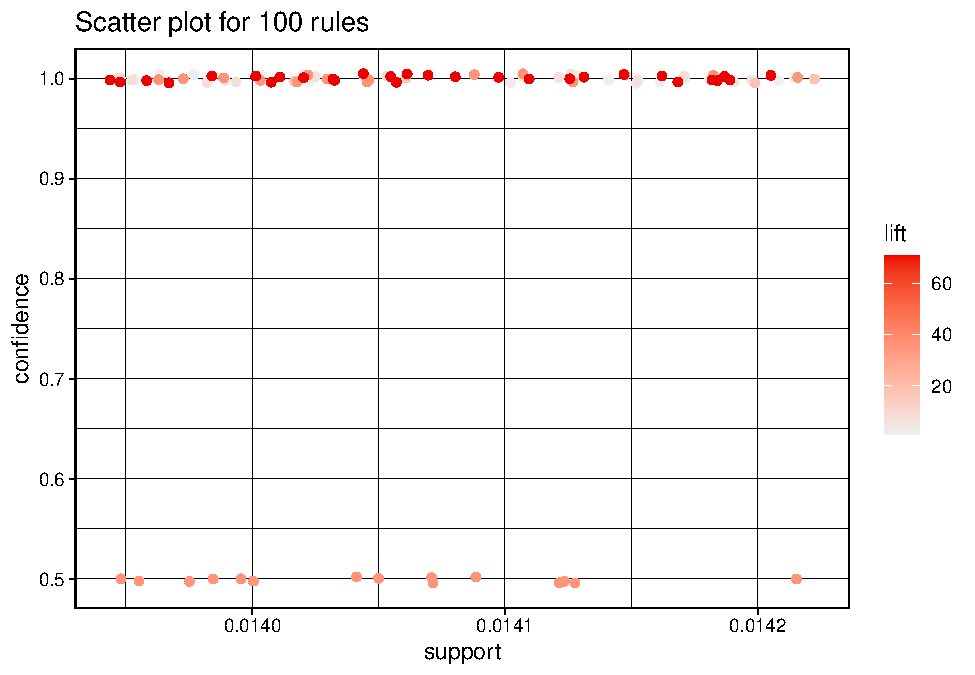
\includegraphics{_main_files/figure-latex/unnamed-chunk-7-1.pdf}

\begin{Shaded}
\begin{Highlighting}[]
\CommentTok{\#plot me crea una grafica}
\FunctionTok{plot}\NormalTok{(cabesa, }\AttributeTok{method =} \StringTok{"matrix"}\NormalTok{)}
\end{Highlighting}
\end{Shaded}

\begin{verbatim}
## Itemsets in Antecedent (LHS)
##  [1] "{scans.McAfee.result=Artemis!433E1FBFF2F2}"                            
##  [2] "{scans.ESET-NOD32.result=a variant of Android/Clicker.KN}"             
##  [3] "{scans.McAfee.result=Artemis!71A0171BCEA9}"                            
##  [4] "{scans.CAT-QuickHeal.result=Android.Hiddad.GEN35225}"                  
##  [5] "{scans.ESET-NOD32.result=a variant of Android/TrojanDropper.Agent.FNN}"
##  [6] "{scans.McAfee.result=Adwind-FDWB.jar!BE68BBB422D0}"                    
##  [7] "{scans.CAT-QuickHeal.result=Android.Agent.GEN36614}"                   
##  [8] "{submission.submitter_country=IN}"                                     
##  [9] "{scans.ESET-NOD32.result=a variant of Android/TrojanDropper.Agent.GZB}"
## [10] "{scans.McAfee.result=Artemis!7D5E9382D046}"                            
## [11] "{scans.CAT-QuickHeal.result=Android.Hiddenad.Abe3a (AdWare)}"          
## [12] "{scans.ESET-NOD32.result=a variant of Android/Hiddad.HI}"              
## [13] "{scans.CAT-QuickHeal.result=Android.Agent.GEN1478}"                    
## [14] "{scans.Lionic.result=Riskware.AndroidOS.Dnotua.z!c}"                   
## [15] "{scans.CAT-QuickHeal.result=Android.Agent.GEN45096}"                   
## [16] "{scans.ESET-NOD32.result=a variant of Android/TrojanDropper.Agent.DMJ}"
## [17] "{scans.Lionic.result=Adware.AndroidOS.HiddenAd.A!c}"                   
## [18] "{scans.CAT-QuickHeal.result=Android.Agent.GEN10334 (PUP)}"             
## [19] "{scans.ESET-NOD32.result=multiple detections}"                         
## [20] "{scans.Lionic.result=Trojan.AndroidOS.Generic.C!c}"                    
## [21] "{scans.ESET-NOD32.result=a variant of Android/TrojanDropper.Agent.IYT}"
## [22] "{scans.McAfee.result=Artemis!A1DCD5D388AF}"                            
## [23] "{scans.CAT-QuickHeal.result=Android.Agent.A5570}"                      
## [24] "{scans.McAfee.result=Artemis!9AA9ED3D4306}"                            
## [25] "{scans.McAfee.result=Artemis!B25E2A555543}"                            
## [26] "{scans.McAfee.result=Artemis!8A04B268C0AD}"                            
## [27] "{scans.McAfee.result=Artemis!FEE8F87A75D1}"                            
## [28] "{scans.McAfee.result=Artemis!C5B53B908443}"                            
## Itemsets in Consequent (RHS)
##  [1] "{additional_info.exiftool.FileType=ZIP}"                               
##  [2] "{submission.submitter_country=CA}"                                     
##  [3] "{scans.Lionic.result=Adware.AndroidOS.Ewind.A!c}"                      
##  [4] "{submission.submitter_country=US}"                                     
##  [5] "{submission.submitter_country=IT}"                                     
##  [6] "{scans.ESET-NOD32.result=Android/SMSreg.UA potentially unsafe}"        
##  [7] "{scans.Lionic.result=Riskware.AndroidOS.SMSreg.z!c}"                   
##  [8] "{scans.CAT-QuickHeal.result=Android.SMSReg.A (PUP)}"                   
##  [9] "{scans.Lionic.result=Trojan.AndroidOS.Bray.C!c}"                       
## [10] "{scans.CAT-QuickHeal.result=Android.SmsThief.GEN44819}"                
## [11] "{scans.ESET-NOD32.result=a variant of Android/Spy.Agent.BMP}"          
## [12] "{scans.ESET-NOD32.result=a variant of Android/TrojanDropper.Agent.IYT}"
## [13] "{scans.Lionic.result=Trojan.AndroidOS.Generic.C!c}"                    
## [14] "{scans.ESET-NOD32.result=multiple detections}"                         
## [15] "{scans.McAfee.result=Artemis!B25E2A555543}"                            
## [16] "{scans.CAT-QuickHeal.result=Android.Agent.GEN10334 (PUP)}"             
## [17] "{scans.Lionic.result=Adware.AndroidOS.HiddenAd.A!c}"                   
## [18] "{scans.ESET-NOD32.result=a variant of Android/TrojanDropper.Agent.DMJ}"
## [19] "{scans.McAfee.result=Artemis!9AA9ED3D4306}"                            
## [20] "{scans.CAT-QuickHeal.result=Android.Agent.GEN45096}"                   
## [21] "{scans.Lionic.result=Riskware.AndroidOS.Dnotua.z!c}"                   
## [22] "{scans.McAfee.result=Artemis!A1DCD5D388AF}"                            
## [23] "{scans.CAT-QuickHeal.result=Android.Agent.A5570}"                      
## [24] "{scans.ESET-NOD32.result=a variant of Android/Hiddad.HI}"              
## [25] "{scans.CAT-QuickHeal.result=Android.Hiddenad.Abe3a (AdWare)}"          
## [26] "{scans.ESET-NOD32.result=a variant of Android/TrojanDropper.Agent.GZB}"
## [27] "{scans.McAfee.result=Artemis!7D5E9382D046}"                            
## [28] "{scans.CAT-QuickHeal.result=Android.Agent.GEN1478}"                    
## [29] "{submission.submitter_country=IN}"                                     
## [30] "{scans.CAT-QuickHeal.result=Android.Agent.GEN36614}"                   
## [31] "{scans.ESET-NOD32.result=a variant of Android/TrojanDropper.Agent.FNN}"
## [32] "{scans.McAfee.result=Adwind-FDWB.jar!BE68BBB422D0}"                    
## [33] "{scans.CAT-QuickHeal.result=Android.Hiddad.GEN35225}"                  
## [34] "{scans.McAfee.result=Artemis!71A0171BCEA9}"                            
## [35] "{scans.ESET-NOD32.result=a variant of Android/Clicker.KN}"             
## [36] "{scans.McAfee.result=Artemis!433E1FBFF2F2}"
\end{verbatim}

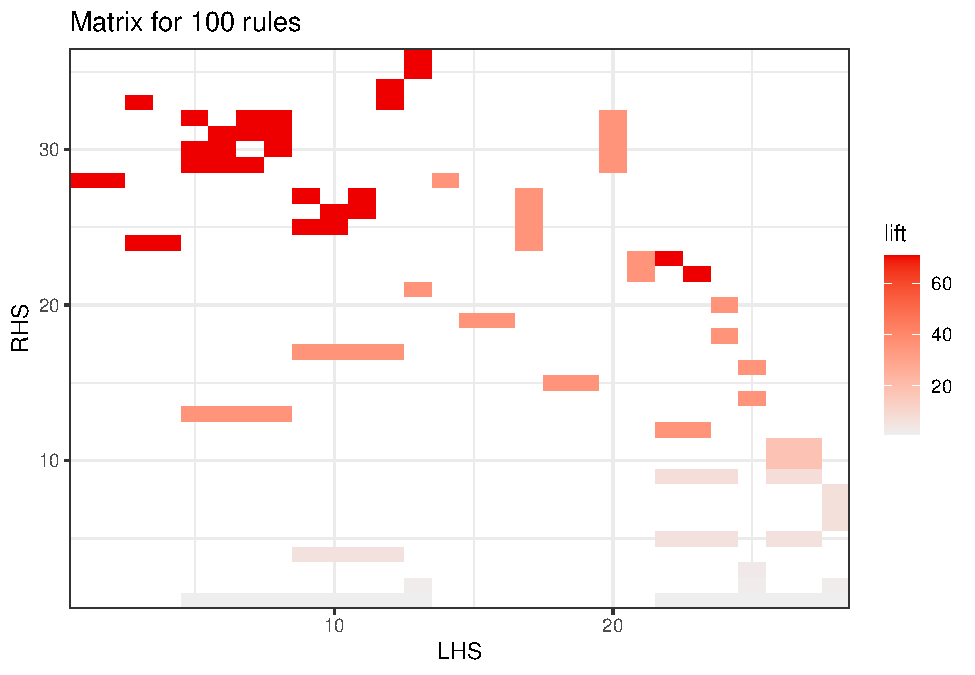
\includegraphics{_main_files/figure-latex/unnamed-chunk-7-2.pdf}

\hypertarget{clusters}{%
\chapter{Clusters}\label{clusters}}

\hypertarget{kmeans}{%
\section{Kmeans}\label{kmeans}}

Haciendo el nbclust nos sale que el valor óptimo de clúster es 2, sin embargo he optado por hacer 5 clústers ya que cuando hacía la visualización quedan mejor agrupados los valores. El resultado se visualiza mediante un gráfico interactivo donde puedes ver el valor de cada nodo con el antivirus al que corresponde.

\begin{Shaded}
\begin{Highlighting}[]
\FunctionTok{fviz\_nbclust}\NormalTok{(}\FunctionTok{t}\NormalTok{(json\_df\_filtrados[,}\DecValTok{4}\SpecialCharTok{:}\DecValTok{45}\NormalTok{]), kmeans, }\AttributeTok{nstart=} \DecValTok{10}\NormalTok{) }
\end{Highlighting}
\end{Shaded}

\begin{verbatim}
## Error in h(simpleError(msg, call)): error in evaluating the argument 'x' in selecting a method for function 't': objeto 'json_df_filtrados' no encontrado
\end{verbatim}

\begin{Shaded}
\begin{Highlighting}[]
\NormalTok{test\_kmeans }\OtherTok{\textless{}{-}} \FunctionTok{kmeans}\NormalTok{(}\FunctionTok{t}\NormalTok{(json\_df\_filtrados[,}\DecValTok{4}\SpecialCharTok{:}\DecValTok{45}\NormalTok{]), }\AttributeTok{centers =} \DecValTok{5}\NormalTok{, }\AttributeTok{nstar=}\DecValTok{100}\NormalTok{)}
\end{Highlighting}
\end{Shaded}

\begin{verbatim}
## Error in h(simpleError(msg, call)): error in evaluating the argument 'x' in selecting a method for function 't': objeto 'json_df_filtrados' no encontrado
\end{verbatim}

\begin{Shaded}
\begin{Highlighting}[]
\NormalTok{grafico\_kmeans}\OtherTok{\textless{}{-}} \FunctionTok{fviz\_cluster}\NormalTok{(test\_kmeans, }\AttributeTok{data =} \FunctionTok{t}\NormalTok{(json\_df\_filtrados[,}\DecValTok{4}\SpecialCharTok{:}\DecValTok{45}\NormalTok{]) , }\AttributeTok{geom=}\FunctionTok{c}\NormalTok{(}\StringTok{"point"}\NormalTok{, }\StringTok{"text"}\NormalTok{))}\SpecialCharTok{+} \FunctionTok{geom\_point}\NormalTok{(}\FunctionTok{aes}\NormalTok{(}\AttributeTok{color=}\NormalTok{cluster, }\AttributeTok{text =}\NormalTok{ name))}
\end{Highlighting}
\end{Shaded}

\begin{verbatim}
## Error in fviz_cluster(test_kmeans, data = t(json_df_filtrados[, 4:45]), : objeto 'test_kmeans' no encontrado
\end{verbatim}

\begin{Shaded}
\begin{Highlighting}[]
\NormalTok{grafico\_kmeans}\SpecialCharTok{$}\NormalTok{layers[[}\DecValTok{4}\NormalTok{]] }\OtherTok{\textless{}{-}} \ConstantTok{NULL}
\end{Highlighting}
\end{Shaded}

\begin{verbatim}
## Error in grafico_kmeans$layers[[4]] <- NULL: objeto 'grafico_kmeans' no encontrado
\end{verbatim}

\begin{Shaded}
\begin{Highlighting}[]
\NormalTok{grafico\_kmeans}\SpecialCharTok{$}\NormalTok{layers[[}\DecValTok{3}\NormalTok{]] }\OtherTok{\textless{}{-}} \ConstantTok{NULL}
\end{Highlighting}
\end{Shaded}

\begin{verbatim}
## Error in grafico_kmeans$layers[[3]] <- NULL: objeto 'grafico_kmeans' no encontrado
\end{verbatim}

\begin{Shaded}
\begin{Highlighting}[]
\NormalTok{grafico\_kmeans}\SpecialCharTok{$}\NormalTok{layers[[}\DecValTok{1}\NormalTok{]] }\OtherTok{\textless{}{-}} \ConstantTok{NULL}
\end{Highlighting}
\end{Shaded}

\begin{verbatim}
## Error in grafico_kmeans$layers[[1]] <- NULL: objeto 'grafico_kmeans' no encontrado
\end{verbatim}

\begin{Shaded}
\begin{Highlighting}[]
\FunctionTok{ggplotly}\NormalTok{(grafico\_kmeans)}
\end{Highlighting}
\end{Shaded}

\begin{verbatim}
## Error in ggplotly(grafico_kmeans): no se pudo encontrar la función "ggplotly"
\end{verbatim}

\hypertarget{dendograma}{%
\section{Dendograma}\label{dendograma}}

Ahora probamos a realizarle un análisis usando un dendograma y luego lo agruparemos en 5 clústers para comprobar si se corresponden con el resultado de kmeans.

\begin{Shaded}
\begin{Highlighting}[]
\NormalTok{distancias }\OtherTok{\textless{}{-}} \FunctionTok{dist}\NormalTok{(}\FunctionTok{t}\NormalTok{(datos\_df\_filtrados))}
\end{Highlighting}
\end{Shaded}

\begin{verbatim}
## Error in h(simpleError(msg, call)): error in evaluating the argument 'x' in selecting a method for function 't': objeto 'datos_df_filtrados' no encontrado
\end{verbatim}

\begin{Shaded}
\begin{Highlighting}[]
\NormalTok{distancias }\SpecialCharTok{\%\textgreater{}\%} \FunctionTok{fviz\_dist}\NormalTok{()}
\end{Highlighting}
\end{Shaded}

\begin{verbatim}
## Error in fviz_dist(.): objeto 'distancias' no encontrado
\end{verbatim}

\begin{Shaded}
\begin{Highlighting}[]
\NormalTok{clusters }\OtherTok{\textless{}{-}}\NormalTok{ distancias }\SpecialCharTok{\%\textgreater{}\%} \FunctionTok{hclust}\NormalTok{()}
\end{Highlighting}
\end{Shaded}

\begin{verbatim}
## Error in hclust(.): objeto 'distancias' no encontrado
\end{verbatim}

\begin{Shaded}
\begin{Highlighting}[]
\FunctionTok{plot}\NormalTok{(clusters, }\AttributeTok{main=}\StringTok{"Detectado Antivirus"}\NormalTok{ )}
\end{Highlighting}
\end{Shaded}

\begin{verbatim}
## Error in plot(clusters, main = "Detectado Antivirus"): objeto 'clusters' no encontrado
\end{verbatim}

\begin{Shaded}
\begin{Highlighting}[]
\FunctionTok{rect.hclust}\NormalTok{(clusters, }\AttributeTok{k=}\DecValTok{5}\NormalTok{ )}
\end{Highlighting}
\end{Shaded}

\begin{verbatim}
## Error in rect.hclust(clusters, k = 5): objeto 'clusters' no encontrado
\end{verbatim}

\begin{Shaded}
\begin{Highlighting}[]
\NormalTok{dendograma }\OtherTok{\textless{}{-}} \FunctionTok{ggdendrogram}\NormalTok{(clusters, }\AttributeTok{rotate =} \ConstantTok{FALSE}\NormalTok{)}
\end{Highlighting}
\end{Shaded}

\begin{verbatim}
## Error in ggdendrogram(clusters, rotate = FALSE): no se pudo encontrar la función "ggdendrogram"
\end{verbatim}

Y ahora mostramos el dendograma en versión interactiva.

\begin{Shaded}
\begin{Highlighting}[]
\FunctionTok{ggplotly}\NormalTok{(dendograma)}
\end{Highlighting}
\end{Shaded}

\begin{verbatim}
## Error in ggplotly(dendograma): no se pudo encontrar la función "ggplotly"
\end{verbatim}

\hypertarget{fca}{%
\chapter{FCA}\label{fca}}

\hypertarget{funciones-para-visualizaciuxf3n-de-fcar}{%
\section{Funciones para visualización de fcaR}\label{funciones-para-visualizaciuxf3n-de-fcar}}

La función plot\_interactivo nos devolverá un objeto plot\_ly donde estará nuestra representación gráfica del fcaR.
En la función plot\_dendograma, dibujará el mapa de calor donde las columnas y las filas estarán ordenadas en función del resultado del dendograma, se le puede pasa opciones de la función heatmap.

\begin{Shaded}
\begin{Highlighting}[]
\NormalTok{plot\_interactivo }\OtherTok{\textless{}{-}} \ControlFlowTok{function}\NormalTok{(fca)\{}
\NormalTok{  matriz\_descompuesta }\OtherTok{\textless{}{-}} \FunctionTok{as.matrix}\NormalTok{(}\FunctionTok{t}\NormalTok{(fca[[}\StringTok{"I"}\NormalTok{]]))}
\NormalTok{  plot\_interactivo }\OtherTok{\textless{}{-}} \FunctionTok{plot\_ly}\NormalTok{(}\AttributeTok{z=}\NormalTok{matriz\_descompuesta, }\AttributeTok{data=}\FunctionTok{as.data.frame}\NormalTok{(matriz\_descompuesta), }\AttributeTok{type =} \StringTok{"heatmap"}\NormalTok{, }\AttributeTok{colors =} \StringTok{"Greys"}\NormalTok{, }\AttributeTok{x=}\FunctionTok{colnames}\NormalTok{(matriz\_descompuesta), }\AttributeTok{y=}\FunctionTok{rownames}\NormalTok{(matriz\_descompuesta))}\SpecialCharTok{\%\textgreater{}\%} \FunctionTok{layout}\NormalTok{(}\AttributeTok{xaxis =} \FunctionTok{list}\NormalTok{(}\AttributeTok{autotypenumbers =}\StringTok{\textquotesingle{}strict\textquotesingle{}}\NormalTok{, }\AttributeTok{type=}\StringTok{\textquotesingle{}category\textquotesingle{}}\NormalTok{), }\AttributeTok{yaxis =} \FunctionTok{list}\NormalTok{(}\AttributeTok{autotypenumbers =}\StringTok{\textquotesingle{}strict\textquotesingle{}}\NormalTok{, }\AttributeTok{dtick=}\DecValTok{1}\NormalTok{ ))}
  \FunctionTok{return}\NormalTok{(plot\_interactivo)}
\NormalTok{\}}
\NormalTok{plot\_dendograma }\OtherTok{\textless{}{-}} \ControlFlowTok{function}\NormalTok{(fca)\{}
\NormalTok{  matriz\_descompuesta }\OtherTok{\textless{}{-}} \FunctionTok{as.matrix}\NormalTok{(}\FunctionTok{t}\NormalTok{(fca[[}\StringTok{"I"}\NormalTok{]]))}
  \FunctionTok{heatmap}\NormalTok{(matriz\_descompuesta, }\AttributeTok{col=}\FunctionTok{c}\NormalTok{(}\StringTok{"White"}\NormalTok{,}\StringTok{"Black"}\NormalTok{))}
\NormalTok{\}}
\NormalTok{plot\_dendograma\_interactico }\OtherTok{\textless{}{-}} \ControlFlowTok{function}\NormalTok{(fca)\{}
\NormalTok{  matriz\_descompuesta }\OtherTok{\textless{}{-}} \FunctionTok{as.matrix}\NormalTok{(}\FunctionTok{t}\NormalTok{(fca[[}\StringTok{"I"}\NormalTok{]]))}
  \FunctionTok{heatmaply}\NormalTok{(matriz\_descompuesta, }\AttributeTok{col=}\FunctionTok{c}\NormalTok{(}\StringTok{"White"}\NormalTok{,}\StringTok{"Black"}\NormalTok{))}
\NormalTok{\}}
\end{Highlighting}
\end{Shaded}

\hypertarget{formal-concepts-analysis}{%
\section{Formal Concepts Analysis}\label{formal-concepts-analysis}}

A continuación voy a aplicar FCA y sacaré la representación del plot de fca en un mapa de calor, usando las funciones de plot\_interactivo, plot\_dendograma y plot\_dendograma\_interactivo. Obtenemos un total de 24 conceptos irreducibles que serían los grupos de antivirus que hay y 75 implicaciones irreducibles que se corresponderían a los grupos de archivos con resultados distintos.

\begin{Shaded}
\begin{Highlighting}[]
\NormalTok{datos\_df\_filtrados }\OtherTok{\textless{}{-}}\NormalTok{ datos\_df\_filtrados}\SpecialCharTok{*}\DecValTok{1}
\end{Highlighting}
\end{Shaded}

\begin{verbatim}
## Error in eval(expr, envir, enclos): objeto 'datos_df_filtrados' no encontrado
\end{verbatim}

\begin{Shaded}
\begin{Highlighting}[]
\NormalTok{atributes }\OtherTok{\textless{}{-}} \FunctionTok{colnames}\NormalTok{(datos\_df\_filtrados)}
\end{Highlighting}
\end{Shaded}

\begin{verbatim}
## Error in is.data.frame(x): objeto 'datos_df_filtrados' no encontrado
\end{verbatim}

\begin{Shaded}
\begin{Highlighting}[]
\NormalTok{json\_df\_filtrados}\OtherTok{\textless{}{-}} \FunctionTok{cbind}\NormalTok{(json\_df\_filtrados[,}\DecValTok{1}\SpecialCharTok{:}\DecValTok{3}\NormalTok{], datos\_df\_filtrados)}
\end{Highlighting}
\end{Shaded}

\begin{verbatim}
## Error in cbind(json_df_filtrados[, 1:3], datos_df_filtrados): objeto 'json_df_filtrados' no encontrado
\end{verbatim}

\begin{Shaded}
\begin{Highlighting}[]
\NormalTok{fc\_detected }\OtherTok{\textless{}{-}}\NormalTok{ FormalContext}\SpecialCharTok{$}\FunctionTok{new}\NormalTok{(datos\_df\_filtrados)}
\end{Highlighting}
\end{Shaded}

\begin{verbatim}
## Error in initialize(...): objeto 'datos_df_filtrados' no encontrado
\end{verbatim}

\begin{Shaded}
\begin{Highlighting}[]
\NormalTok{fc\_detected}\SpecialCharTok{$}\FunctionTok{clarify}\NormalTok{()}
\end{Highlighting}
\end{Shaded}

\begin{verbatim}
## Error in eval(expr, envir, enclos): objeto 'fc_detected' no encontrado
\end{verbatim}

\begin{Shaded}
\begin{Highlighting}[]
\NormalTok{fc\_detected}\SpecialCharTok{$}\FunctionTok{reduce}\NormalTok{()}
\end{Highlighting}
\end{Shaded}

\begin{verbatim}
## Error in eval(expr, envir, enclos): objeto 'fc_detected' no encontrado
\end{verbatim}

\begin{Shaded}
\begin{Highlighting}[]
\NormalTok{fc\_detected}\SpecialCharTok{$}\FunctionTok{plot}\NormalTok{()}
\end{Highlighting}
\end{Shaded}

\begin{verbatim}
## Error in eval(expr, envir, enclos): objeto 'fc_detected' no encontrado
\end{verbatim}

\begin{Shaded}
\begin{Highlighting}[]
\NormalTok{fc\_detected}\SpecialCharTok{$}\FunctionTok{find\_concepts}\NormalTok{()}
\end{Highlighting}
\end{Shaded}

\begin{verbatim}
## Error in eval(expr, envir, enclos): objeto 'fc_detected' no encontrado
\end{verbatim}

\begin{Shaded}
\begin{Highlighting}[]
\NormalTok{fc\_detected}\SpecialCharTok{$}\FunctionTok{find\_implications}\NormalTok{()}
\end{Highlighting}
\end{Shaded}

\begin{verbatim}
## Error in eval(expr, envir, enclos): objeto 'fc_detected' no encontrado
\end{verbatim}

\begin{Shaded}
\begin{Highlighting}[]
\NormalTok{fc\_detected}\SpecialCharTok{$}\FunctionTok{standardize}\NormalTok{()}
\end{Highlighting}
\end{Shaded}

\begin{verbatim}
## Error in eval(expr, envir, enclos): objeto 'fc_detected' no encontrado
\end{verbatim}

\begin{Shaded}
\begin{Highlighting}[]
\NormalTok{fc\_detected}\SpecialCharTok{$}\NormalTok{implications}
\end{Highlighting}
\end{Shaded}

\begin{verbatim}
## Error in eval(expr, envir, enclos): objeto 'fc_detected' no encontrado
\end{verbatim}

\begin{Shaded}
\begin{Highlighting}[]
\NormalTok{mapa\_calor }\OtherTok{\textless{}{-}} \FunctionTok{plot\_interactivo}\NormalTok{(fc\_detected)}
\end{Highlighting}
\end{Shaded}

\begin{verbatim}
## Error in h(simpleError(msg, call)): error in evaluating the argument 'x' in selecting a method for function 'as.matrix': error in evaluating the argument 'x' in selecting a method for function 't': objeto 'fc_detected' no encontrado
\end{verbatim}

\begin{Shaded}
\begin{Highlighting}[]
\NormalTok{mapa\_calor}
\end{Highlighting}
\end{Shaded}

\begin{verbatim}
## Error in eval(expr, envir, enclos): objeto 'mapa_calor' no encontrado
\end{verbatim}

\begin{Shaded}
\begin{Highlighting}[]
\FunctionTok{plot\_dendograma}\NormalTok{(fc\_detected )}
\end{Highlighting}
\end{Shaded}

\begin{verbatim}
## Error in h(simpleError(msg, call)): error in evaluating the argument 'x' in selecting a method for function 'as.matrix': error in evaluating the argument 'x' in selecting a method for function 't': objeto 'fc_detected' no encontrado
\end{verbatim}

  \bibliography{book.bib,packages.bib}

\end{document}
